\chapter{Adapting Sustainable Agile for Kvanttori Case}\label{chapter5}
This chapter explores how agile software development is currently implemented at Kvanttori, what Kvanttori wants to achieve with a sustainable agile model, how to create and implement such a model, and how it differs from the current agile model at Kvanttori. This chapter answers \textbf{RQ3: How to integrate sustainable development methods into an agile development process?} by adding methods and criteria in Chapter~\ref{chapter2}, parts of different agile models in Chapter~\ref{chapter3}, and metrics and tools in Chapter~\ref{chapter4} to the current development model at Kvanttori.

\section{How Kvanttori Implements Agile}\label{currentimplementation}
The development model described in this section was created by gathering information from Kvanttori's internal development guides and by personally having worked on different projects at Kvanttori.

Kvanttori's current agile implementation is based on Scrum using Essential Scrum~\cite{essentialscrum} as a guidebook for applying Scrum during the development process. The process implements all parts of the Scrum framework as pictured in Figure~\ref{scrumprocess} in Section~\ref{scrum} as well as some additional parts from the Essential Scrum book. The current process is illustrated in Figure~\ref{kvanttoriagile}. The process is split into four sections: pre-development, development, usage, and post-development. Usually, the project starts with pre-development with development and usage happening at the same time when the project is in active development. Post-development phase happens after the project ends or moves into maintenance mode. The maintenance usually entails working on bug fixes and updating dependencies when needed. It can also include monitoring and fixing issues with the hosting environment as needed. Earlier phases can be revisited as necessary. Introducing a new feature might require new technologies to be evaluated and projects can return from maintenance to active development.

Currently, the development process does not take performance and other factors correlating with \gls{environmentalsustainability} into account as long as they are not part of the customer requirements. Only if some features must happen in a specific time limit or if performance is detrimental to usability, will it be used as a reason to not accept a feature as done. \Gls{economicalsustainability} is mostly the responsibility of the customer in the current model as costs are reported directly to the customer but following them and actively minimizing them is not prioritized over other tasks as long as they stay within the customer's budget. \Gls{technicalsustainability} is measured in the backlog using labels for defects in software but bugfixes and refactors are not systematically prioritized and can often stay in the backlog for a long time if not deemed critical.

\begin{figure}[H]
\caption{Kvanttori's current agile implementation}
\label{kvanttoriagile}
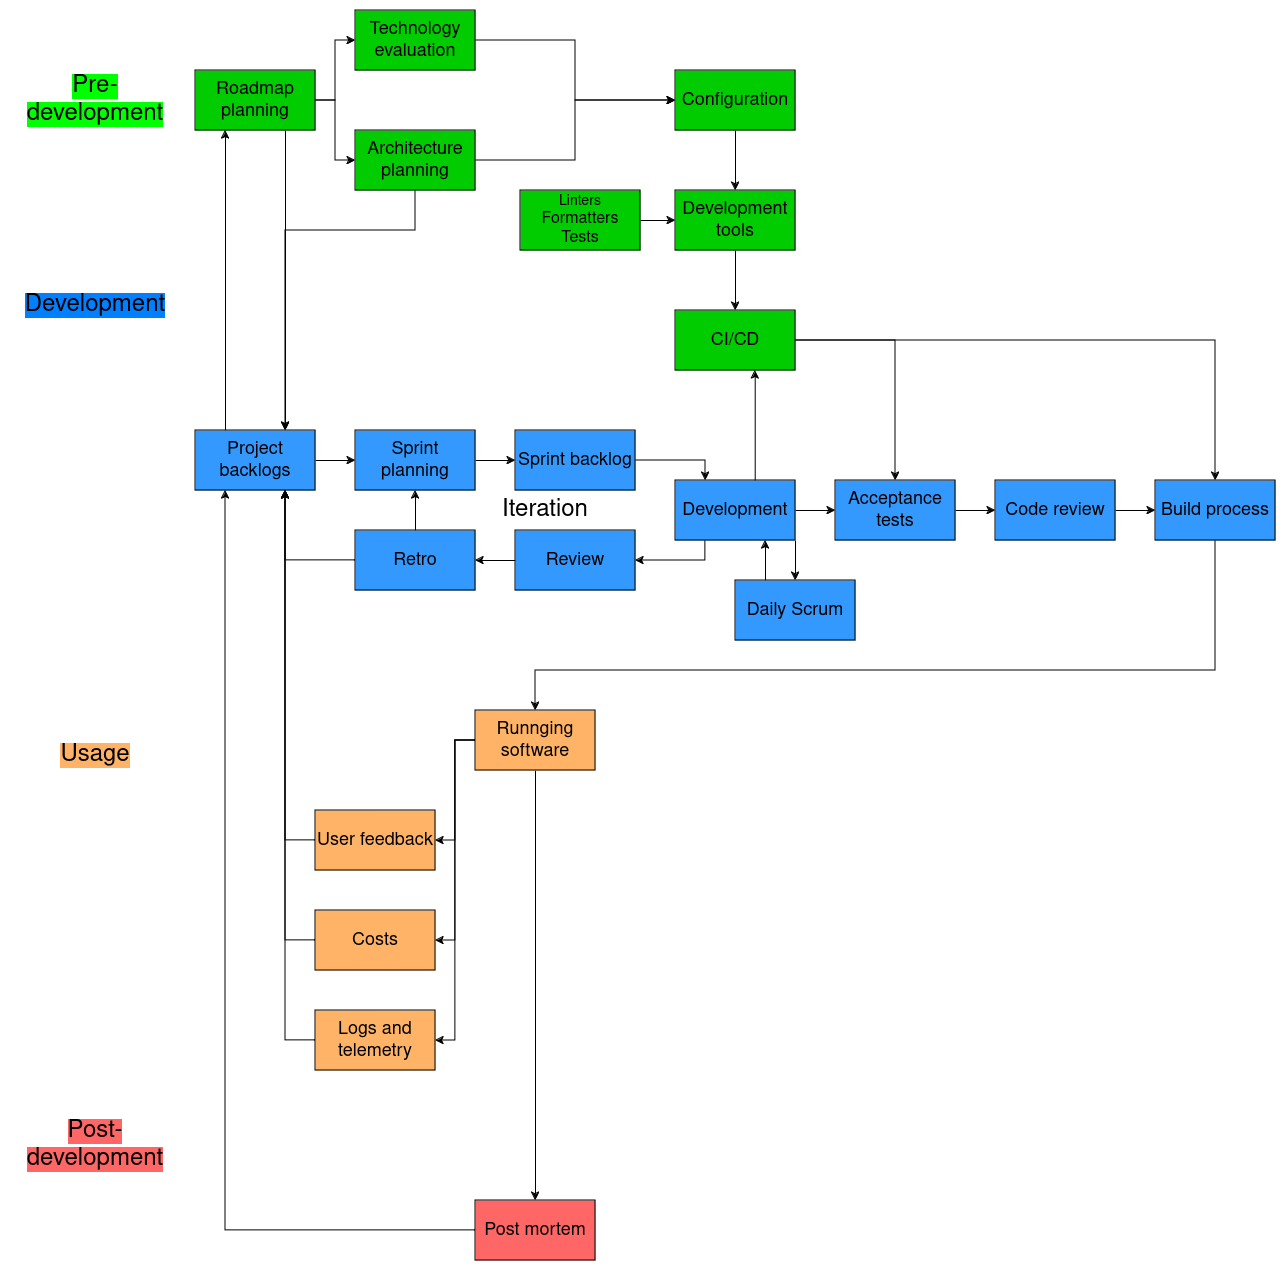
\includegraphics[width=\textwidth]{images/currentagile.png}
\centering
\end{figure}

\subsection{Pre-development Phase}
Pre-development phase consists of setting up the project, finding out high-level requirements, choosing technologies, and setting up the development environment.

\subsubsection{Roadmapping}
Projects start by meeting with a customer to get a better understanding of the customer's business and the problem that needs to be solved. During these meetings, high-level requirements are gathered for the software solution to be developed during the project. This entails estimating how many sprints there will be, how long they are, deadlines imposed by the customer, how releases are done, and estimated work required for the most central features. This is expected to change during the development process but it is used as a starting point for determining what big features are the most important. These features or epics will be split into smaller stories during development. This implements envisioning and release planning from the Essential Scrum~\cite{essentialscrum}.

\subsubsection{Technology Evaluation}
Technologies for a project are chosen based on customer and technical requirements such as previous technology used, platform support, and library ecosystem. The familiarity of the development team with technologies is also considered.

\subsubsection{Architectural Planning}
Architectural planning takes into account any customer requirements for existing systems interoperability with the software being developed as well as the needs of the software being developed.

Architectural planning also includes the distribution and hosting of the software. The choice of hosting methods and hosting provider is affected by the customer's existing systems, the need for scalability, costs, and the skill set of the development team.

\subsubsection{Configuration, Development Tools and CI/CD}
The configuring step is for setting up the necessary development tools and CI/CD pipelines for automated testing and releases.

All projects use linters, formatters, and testing tools to ensure the quality and readability of the code and to ensure the software is working as expected. These are chosen by the lead developer depending on the project and technologies used and are often integrated directly into the development environment as well as CI/CD pipelines.

\subsection{Development Phase}
The day-to-day development process follows Scrum closely including daily Scrum, sprint planning, retro and review steps. Kvanttori uses story points and planning poker together with project management tools to estimate and track team velocity.

Project backlogs are used to keep track of work to be done for the project. This is implemented with a Kanban~\ref{kanbanmethod} board that allows labeling use of stories with labels such as features or bugs.

Sprint planning is used to estimate story points and choose stories from the project backlog to the sprint backlog. The chosen stories depend on the stakeholder requirements as well as the amount of points assigned to each task.

Sprint backlog tracks work that needs to be done in the current sprint. This is implemented with the same tool as the project backlog.

Acceptance tests are automatically run in CI/CD pipelines to ensure compliance with formatting, linting, and tests.

Code review is conducted by other team members, often by the lead developer to ensure the quality of implementation and compliance with high-level architecture.

\subsection{Usage Phase}
Logs are collected from the software to find errors that users may run into and add fixing them to the product backlog. Telemetry may also be implemented to find what features are used the most but is not required.

\subsection{Post-development Phase}
Lastly, after the project ends, there is a post-mortem of the project where things learned from the project are discussed among the development team and written for other development teams to read for future projects.

\subsection{Roles}
Kvanttori has four roles in the development team with one person sometimes having multiple roles. These are Product owner, Scrum master, lead developer, and developer. With one person often taking on multiple roles due to team sizes. For example, the Product owner can also be the lead developer and the Scrum master is often also a developer. The lead developer is a role that is not specified in Scrum roles but has been deemed useful at Kvanttori based on experiences in different projects.

\section{Sustainable Agile Implementation}\label{susimplementation}
The sustainable agile model described in this section was created by implementing findings of the literature review including methods for creating sustainable software in Chapter~\ref{chapter2}, existing agile and sustainable agile methods in Chapter~\ref{chapter3}, and metrics and measurement tools in Chapter~\ref{chapter4} into the current development model used at Kvanttori presented in Section~\ref{currentimplementation}.

Kvanttori wants a model that allows it to create software that is more sustainable technically, economically, and also environmentally. The model should also aim to prevent the accumulation of \gls{sustainabilitydebt}~\cite{sustainabilitydebt} including technical sustainability debt, economical sustainability debt, and environmental sustainability debt. In addition, the model helps standardize the development model to ensure that teams have a checklist of issues to take into account in every project. This model should aim to include all methods for improving the sustainability of software presented in Section~\ref{methods} as well as issues raised in Chapter~\ref{chapter3} green agile models such as measuring and reporting sustainability, reducing waste in software and allow users to use software in more sustainable ways. The model should also implement metrics discussed in Section~\ref{susmetrics}. The result of using the proposed model should be software that is cheaper to develop and run, uses less energy, is faster, and is easier to maintain.

The new model retains the four phases of the current model, those being pre-development, development, usage, and post-development. Similarly to the current model, these phases can be revisited multiple times during development.

Some new steps and metrics for the development model are required to ensure that sustainability is taken into account during all phases of the development model. In addition, some existing steps and roles have been changed to better take sustainability into account. Figure~\ref{greenagile} illustrates the proposed process model.

\begin{figure}[H]
\caption{Proposed sustainable agile implementation model}
\label{greenagile}
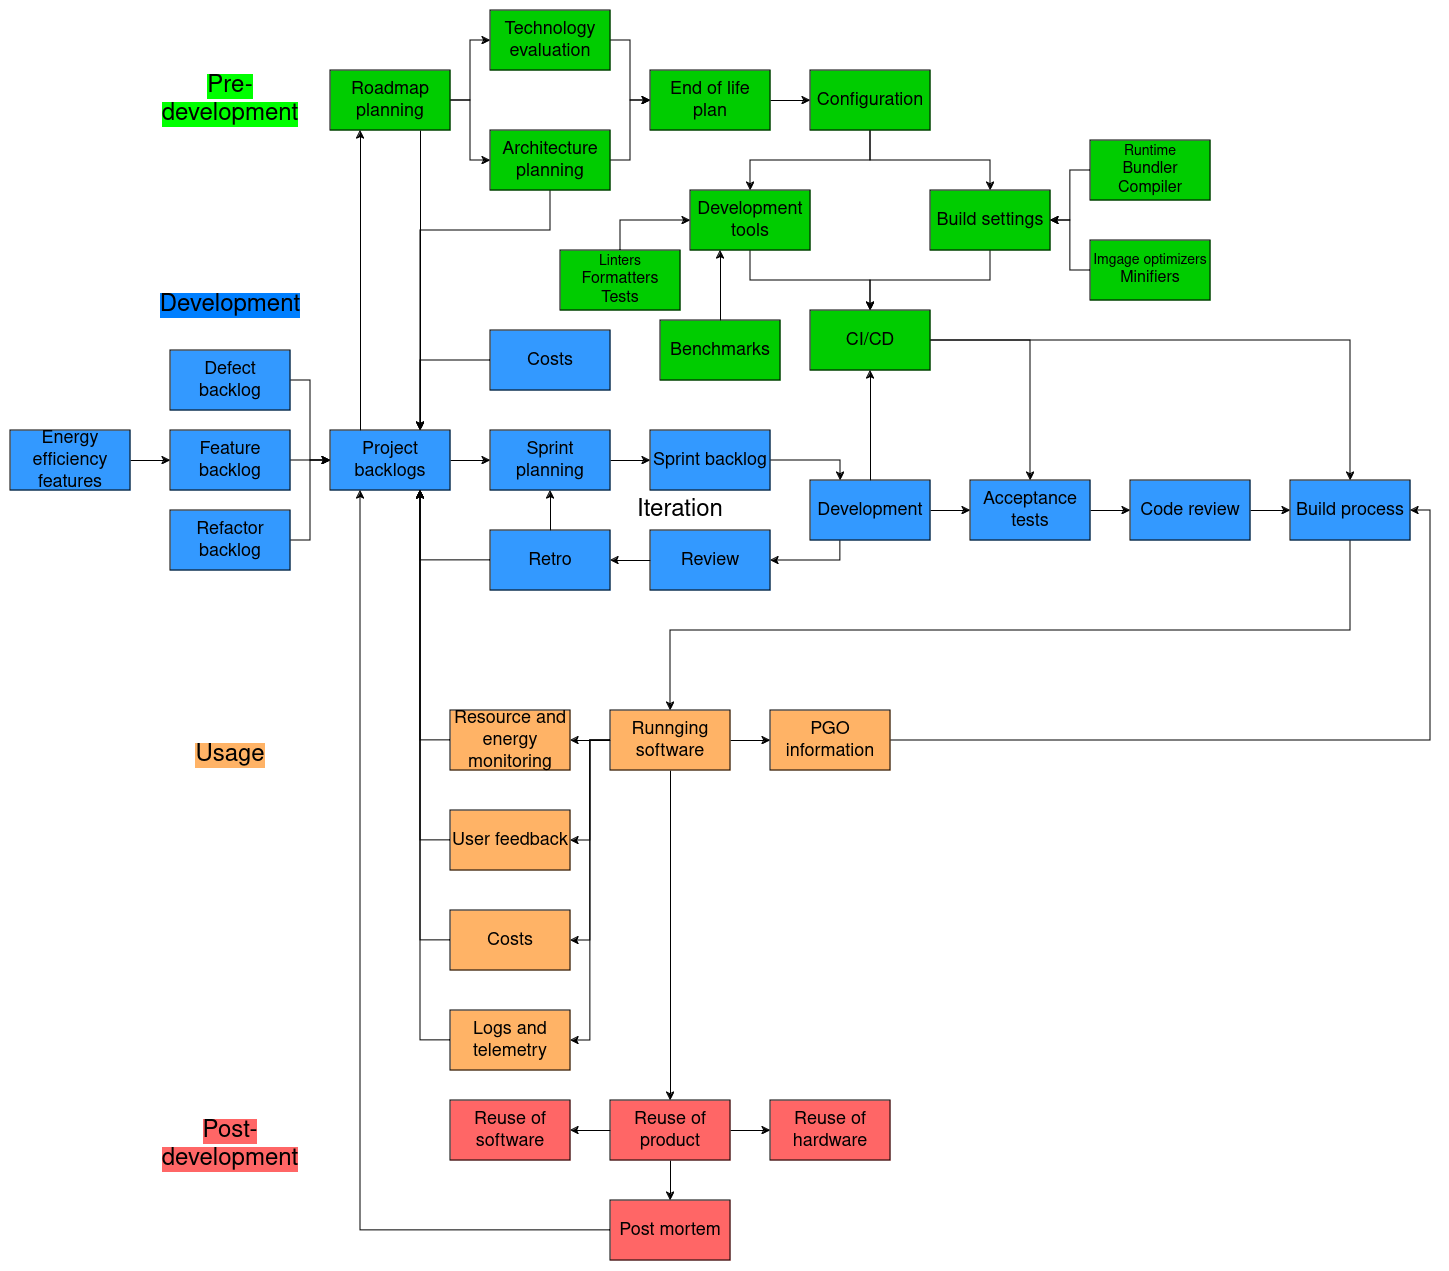
\includegraphics[width=\textwidth]{images/greenagile.png}
\centering
\end{figure}

\subsection{Pre-development Phase}
Many steps can be taken at the beginning of the project that can facilitate a more sustainable development process and end product. These steps often need to be done once per project and sometimes updated during the course of the project but can still have a great impact on the sustainability of the software.

\subsubsection{Roadmapping}
Roadmapping stays mostly the same as in the current model. The core functionality of the product is discussed with the customer and a high-level roadmap is created for the product depending on the feature priorities. These features are then split into epics, which will be further split into user stories. The purpose of this roadmap represent the overall vision for the product and to ensure the project stays true to this vision and does not start adding unnecessary features during development. The roadmap should answer the question of why this software exists. If this question can not be answered, the development should be stopped and the necessity reevaluated as it is the most efficient to not develop anything that is not needed. 

The roadmapping step partially implements the requirements engineering of the Green model for sustainable software engineering shown in Section~\ref{greenmodelforsustainable} by helping determine if the software should be built to solve the problem of the customer. It also creates an outline of the services and features as a roadmap. Risk analysis in terms of energy usage is left out as there is no way to accurately estimate energy usage this early in the project. Requirements testing is also left out as the requirements presented here are meant to indicate what the product needs to do on a high level, meaning they can well be changed during the development.

\subsubsection{Architectural Planning}
The architecture of the software should be planned so that it is extensible enough that features can be easily added but are not too complex. The architecture plan should account for the architecture of the whole software stack including frontend, backend, databases, and hosting platform as well as the architectures of these parts individually. The result of this should be a document describing the high-level architecture of the software stack as well as the high-level architectures of the individual parts of the stack.

Section~\ref{architecture} introduced the following considerations for the architecture of software from a sustainability perspective: \textbf{Caching} and \textbf{bulk requests}, \textbf{data structures and algorithms}, \textbf{error handling}, \textbf{logging}, \textbf{offloading}, and \textbf{indexing}. Many choices made during architectural planning are likely to reappear in day-to-day development work and should follow the same principles as outlined in this step.

%Cache and bulk
\textbf{Caching} should be implemented in all levels of software if possible meaning for example that the database should cache indexes and specific query results, backend should cache expensive function results, database query results, and external API results. Frontend should also cache the results of requests to the backend and possible requests to external APIs. Backend and databases should be planned in such a way that clients can fetch all relevant information with as few queries as possible. This can be achieved with good planning and utilizing \textbf{bulk requests}.

% Data structures and algorithms
Some \textbf{data structures and algorithms} can already be decided during the architecture planning of the software. For data structures, these decisions should account for the most common use cases and optimize for access, search, insertion, or deletion speed based on the use cases. The same applies to algorithms. Decisions on what algorithms are used should take the use case into account and in cases such as password hashing algorithms, find a balance between security and required computation. For both data structures and algorithms optimizing for speed is more important than optimizing for memory.

% Error handling
Architecture should also include details such as how \textbf{errors are handled}. While error handling is largely dependent on the chosen languages and error handling paradigms used by them, there should be some outline of how the errors are propagated through the software and gracefully handled to prevent unexpected errors from crashing the software. 

% Logs
In addition, the architecture should outline what should be \textbf{logged} in the software to catch helpful information about errors and usage. Good logs are vital for finding issues with the software but not everything should be logged as outlined in Section~\ref{logs}. At a minimum, any errors and relevant context to their occurrence should be logged. Any additional logs should be carefully reviewed to determine their usefulness.

% Indexing
Architecture should also outline what should be \textbf{indexed} in databases when planning the initial database schemas to ensure the database operates with optimal performance. Any fields that are frequently used to search for items in the database should be indexed.

% Offloading
\textbf{Offloading} specific computationally intensive work to a server can benefit the client application by lowering system requirements and also allow for more centralized caching of computationally intensive calculations. This should also be accounted for in the software architecture.

% Hosting
Infrastructure architecture should take into account the features that will be added according to the roadmap and ensure the chosen infrastructure is scalable for the expected amount of users for the software. Costs are also an important factor as some infrastructure options might be initially sufficient and cheap but become expensive when scaling up. Developer familiarity with platform options is key in predicting these costs and should therefore be a factor when choosing hosting platforms and methods. The choice of service provider should also be affected by how they produce their energy and other factors mentioned in Section~\ref{hosting}. This will not likely have an impact on the energy consumption of the software but it ensures that the energy consumed is produced responsibly. Hosting platforms also provide varying levels of metrics on energy consumption and using the platform with the most accurate tools should be considered if possible within other requirements.

This phase implements the design and implementation stages of the green model for sustainable software engineering in Section~\ref{greenmodelforsustainable} by creating a system architecture based on the requirements and guidelines for producing more sustainable software.

\subsubsection{Technology Evaluation}
The technology used for a project often depends on customer requirements such as compatibility and performance and also on potential earlier development work. Section~\ref{technology} outlined different technological decisions affecting the energy consumption of the application. These were \textbf{Programming language}, \textbf{runtime}, \textbf{databases} and \textbf{libraries and frameworks}, and \textbf{large language models}. This step should consider all those decisions.

% Limitations
Platform support can affect what technologies can be used for the project for example not all languages and frameworks are suitable for mobile development or embedded systems. If desired platforms do not have an operating system, using low-level languages such as C or Rust is often required.

% Languages
Faster \textbf{programming languages} allow using less powerful hardware to serve the same amount of users as less performant languages with more powerful hardware which also saves in hosting and usage costs making it more sustainable both economically and environmentally. Performance is also especially important on serverless functions platforms as they are often billed by usage time. On serverless platforms, the startup time of the software is crucial for ensuring users do not need to wait too long when using an application. Using performant technologies also allows for higher scaling for lower prices.

% Runtimes
Even if the language used is not the most efficient such as many interpreted languages, the choice of \textbf{runtime} can significantly improve the performance and by extension energy consumption. For example, JavaScript developers should consider Bun as runtime instead of Node due to it being more efficient as mentioned in Section~\ref{runtime} while not being that different from using NodeJs in practice.

% Error handling
Another consideration is how a language or framework handles errors. Making as many errors recoverable as possible is usually better than crashing and restarting the application. To this end technologies that use errors as values and are null safe should be considered provided the team is proficient with them as they can help developers make sure all errors are handled and reduce the rate of unexpected crashes. These kinds of technologies can help enhance technical sustainability by making the software more resilient and also easier to refactor as many issues are caught during the build process.

% Dev familiarity
The current development team's expertise in technologies should also be considered. The development team should choose the most efficient technology they are familiar with and that supports the desired target platforms for the software and configure those technologies to be as efficient as they can. Using familiar technologies allows the team to make better quality software making it more technically sustainable.

% Databases
The choice of \textbf{database} often depends on the use case. However, for most cases at least at the beginning of a project a SQL database such as Postgres or MySQL is sufficient and provides good performance and technical maintainability, especially with proper indexing. SQL databases are also well-supported in most cloud platforms and have solid library support in most languages.

% Libraries
\textbf{Libraries and frameworks} should be carefully considered as they can introduce a lot of unnecessary bloat to software. Libraries should accomplish some specific task and the smallest but still actively maintained library should be used. In cases where only some functionality from a large library is needed, it might make sense to only implement the required functionality. Unnecessary libraries were noted to be detrimental in A Green Model for Sustainable Software Engineering in Section~\ref{greenmodelforsustainable}.

In the case of frameworks, first, it should be evaluated if a framework is even needed. If it is, the choice should be based on performance and available features, not just on what the development team has previously used. Unlike new languages, the time required to learn framework-specific features is often much shorter if the language used in the framework is familiar to the developers.

% LLMS
As mentioned in Section~\ref{llm}, some technologies such as \textbf{large language models} can consume large amounts of energy and there are considerations when using them. For LLMs, the smallest model that fits the requirements should be used. The usage of these technologies should also be carefully considered as more traditional approaches can often be sufficient.

\subsubsection{End of Life Plan}
Software products should have a plan for when they are eventually deprecated and the data needs to be migrated to different platforms. There should be a plan that includes how to export the data used by the software, what format the data is in, and who can export the data. Open data formats should be used to make the data export and reuse easier. It should also include what will be done with the current software in case of end-of-life. Will it be partially reused, open-sourced, or just thrown away? This plan can change throughout the software lifecycle but thought should be given to this as it will likely affect how development is conducted. For example, if the plan is to eventually open source the project, special attention needs to be paid to not use any proprietary code or other media that cannot be open-sourced. Open sourcing specifically should be considered as even if current users might eventually not need the software, someone else can benefit from it and it might even lead to them not needing to develop another comparable product themselves.

\subsubsection{Configuration}
Depending on the technologies used, different configuration options can be used to drastically improve the performance and resource usage of the application as mentioned in Section~\ref{configuration}. Out of the box, many languages have a separate development mode for fast builds and iterations and a production mode for faster runtime performance and smaller bundle sizes. However, these configurations can often be further improved for specific situations and developers should not rely on default options being the best for their use case. During the configuration step, the target platform should be taken into account, and configure the software to be as performant on that platform as possible. If the target platform is a browser or embedded device, it might make sense to optimize for size to ensure minimal network traffic or to ensure that the program can fit the device.

\subsubsection{Development Tools}
Different development tools such as linters and formatters should be used to improve overall code quality and consistent formatting of the code. Running these tools locally also reduces unnecessary CI/CD runs as the code is already compliant with formatting and linting settings enforced in CI/CD pipelines.

Developers can also use tools to assist in writing more efficient software. These tools should present minimal overhead for the developer. This is often achieved by integrating these tools directly with the editors. Static code analyzers are great for integrating with build pipelines as well as the developer's development environment. While tools for directly finding energy patterns in code are still lacking, tools for writing more performant code exist. Depending on the technology used, there are tools such as SonarLint~\cite{sonarsourceLinterTool} that can give hints on writing more performant software. These kinds of tools should be known and recommended in projects by the lead developer depending on the technologies used. They should also be included in the CI/CD pipelines to enforce compliance with them.

Tests should be used to help maintain code quality by detecting issues as early as possible. There are many types of tests such as unit tests, integration tests, end-to-end tests, and testing methods such as property-based testing and fuzzing. Relevant testing approaches are determined by the nature of the project and should be chosen so that they help in detecting issues in the software but do not cause unnecessary overhead to developers.

Benchmarks can be used to catch regressions in the performance of the application or enforce limits on certain features based on what is acceptable according to customer needs or the definition of done. Performance correlates strongly with energy consumption and therefore this can be useful in estimating changes in energy consumption of a specific part of the software. Benchmarks, like tests, can be used as part of the definition to prevent new features and changes from raising the execution time of some features more than is acceptable. They can also be included in CI/CD pipelines to follow changes in performance and energy consumption~\cite{twinsorfalseffriends}.

\subsubsection{Build Settings}
\gls{pgo} is a technique that can be used to improve performance in some compiled languages by compiling software with it enabled, collecting produced data from the production environment, and feeding it back to the compiler during the build step. This allows the compiler to make use case-specific optimizations to the software.

% External tools
For many technologies, there are additional tools to make the final product more efficient. Image optimizer tools such as sharp~\cite{pixelplumbingSharpHigh} can be used to automatically convert PNG and JPEG images to newer formats such as AVIF and WEBP during the build process as well as compress images without noticeable quality loss. For web assembly, there are minifier tools such as wasm-opt~\cite{githubGitHubWebAssemblybinaryen} that can be used to reduce the size of the wasm files during the build process. These tools should be set up at the beginning of the project and used in CI/CD pipelines as part of the build process. For JavaScript and Typescript, many bundlers already perform minimization for code and style files. These techniques can be used to make web applications load faster and reduce network traffic.

\subsubsection{CI/CD}
% CI/CD and Development tools
CI/CD pipelines should also be set up at the start of the project to run chosen tools on pull requests. These tools can include testing frameworks, benchmarks, formatters, linters, and other static analyzers. CI/CD pipelines should be configured to use caching for build artifacts and dependencies to keep them from needing to redownload and recompile on every run. Pipelines should also run the fastest tests and tools first and stop running if any tools fail as this prevents running all tools if the result of the combined tests is a failure.

% Unused dependencies
Unused dependencies should be checked as part of testing and release pipelines and removed from the project. Unused dependencies can, depending on the technologies used, slow the software, bloat the bundle size, or increase compile and therefore pipeline execution times. They also cause unneeded network and I/O usage during building as dependencies are downloaded and installed. There are tools for detecting unused dependencies for most major languages. These tools should be integrated into the CI/CD pipeline to check for unused dependencies. Removing unused dependencies is part of reducing the waste defined in Section~\ref{waste} of the software by removing unneeded features from it.

% Dependency vulnerabilities
Automated tools should also be used to catch dependencies that have vulnerabilities so they can be addressed. This is mostly useful for security but also indirectly saves energy as handling issues caused by possible exploitation of these vulnerabilities is sure to consume more energy than patching them preemptively.

% Specialized tools
Tools such as Google's Lighthouse can be run in CI/CD pipelines for web applications to detect performance, accessibility, and SEO issues in front-end applications. The viability of these kinds of specific tools often depends on the nature of the project.

Some tests could also be run only when things relating to them have changed and on some commits, tests could be skipped altogether~\cite{skippedcommits}. For example, all tests should not be run if only some documentation files were updated. Similar to extreme programming presented in Section~\ref{xp}, the build and testing pipeline should take at most 10 minutes. The 10-minute mark can be used as a heuristic that something is wrong with the performance of the pipeline and it should be addressed.

\subsection{Development Phase}
These steps are done once or more times during every iteration, therefore it is important to avoid adding too many things here so as not to distract from the actual development work. Daily scrum was also dropped as a requirement since many teams within Kvanttori have noticed that it does not bring any benefit and serves as an unneeded distraction from actual work as the same effect can be achieved with communication tools used by teams. This observation is likely due to the development team sizes at Kvanttori being often relatively small. Teams may implement this if they feel it is beneficial.

This phase together with the pre-development phase corresponds to the development phase in the Greensoft model's lifecycle of software products in Section~\ref{greensoft}.

\subsubsection{Backlogs}
Backlogs are used to keep track of work that needs to be done. The product backlog keeps track of all the work while the sprint backlog shows work that has been picked for the current sprint. The product backlog is split into feature, defect, and refactor backlogs. Kanban board presented in Section~\ref{kanbanmethod} can be used to implement these backlogs, as many Kanban tools allow separating backlog into different sections such as labels or lanes.

% Feature backlog
Feature backlog keeps track of new features that need to be added to the product. These items are often added due to customer or other stakeholder requirements. Items can be also added to enhance the energy efficiency of the software. Such features could be based on the criteria presented in Section~\ref{criteria}. This also partially implements the usage stage of the green model for sustainable software engineering in Section~\ref{greenmodelforsustainable} by implementing features that enhance energy efficiency.

% Refactor backlog
A separate refactor backlog ensures that potential refactors do not get prioritized as is often the case if they share the backlog with features. Developers should keep an eye out for potential refactoring opportunities and streamlining of functionality on features done earlier in the project to ensure the project does not become too complex and accumulate technical debt. There is research suggesting that some refactors can improve the energy efficiency of software~\cite{refactorforenergyefficiency}. There seems to be a problem where the need for refactors is recognized during the project but no time is given to do them as they do not seem to immediately give value to the customer. These slowly accumulate technical sustainability debt and make adding new features harder to do correctly without workarounds~\cite{sustainabilitydebt}. Any potential refactors should be reported to the product owner who will then add them to the refactor backlog. If there are items in the refactor backlog, at least 10\% of the sprint effort must be spent on those items to ensure that architectural, technical, and sustainability debt cannot accumulate in the software. In addition to developer feedback, adding items to the refactor backlog is informed by customer feedback and energy and resource usage reported by the hosting environment of the application in addition to error logs and telemetry data collected from the hosting environment.

% Defect backlog
A separate backlog for defects in software should also be set up. This is important to keep track of the \gls{technicalsustainability} of the project and ensure defects cannot accumulate in software. As with refactor backlog, at least 10\% of sprint effort should be spent on fixing defects and as with refactor backlog, the percentage will likely change during the project depending on the speed defects are accumulating.

\subsubsection{Development and Energy Efficient Choices}
% UI design
Section~\ref{methods} outlined methods for ensuring UI design facilitates more efficient software. The UI/UX design should try to minimize the amount of actions required from the user to perform some task within the software. Dark colors should be preferred for better energy efficiency with OLED displays. Visual elements such as animations should also be used sparingly.

Accessibility also needs to be taken into account to improve the software's energy efficiency. If the software does not support accessibility tools such as screen readers, the likelihood of misinputs by users relying on those tools increases which in turn increases the energy usage of the application. The minimum requirement for front-end applications should be the Google lighthouse accessibility check.

% Data structures and algorithms
There will likely be many times during the development when developers need to choose data structures and algorithms to solve a specific problem or to add some feature. These decisions should use the same criteria as the architecture planning step. That is, choose the algorithms based on the use case, prefer lower time complexity over lower space complexity, and find a balance between usability and robustness. The same applies to other part of the architecture planning. Adding new indexes to the database, creating features that make requests to the database or external services, or adding error handling to new features should follow the patterns outlined in the architecture planning step and enforced by the lead developer during code reviews.

This step partially implements the usage stage of the green model for sustainable software engineering in Section~\ref{greenmodelforsustainable} by making software as simple as possible to allow users to perform as few actions as possible to achieve a specific task with the software.

\subsubsection{Acceptance tests}
Tests and other development tools such as formatters and linters that have been set up during the pre-development phase and those added later during the development should be automatically run on code pull requests to enforce code quality.

This step implements the testing stage of the green model for sustainable software engineering in Section~\ref{greenmodelforsustainable} by discovering defects in software before taking it to production. This also partially implements the analysis stage as benchmarks are run during this step.

\subsubsection{Code review}
During code review the lead developer should review the code and ensure it follows the architecture created during the architecture planning and also make sure the code follows sustainable software principles such as using caching, correct data structures and algorithms, and handling error cases properly.

\subsubsection{Review}
In addition to the current model's review step, stakeholders should be made aware of the different measurements collected during the projects such as costs, energy and resource usage, and \gls{technicalsustainability} metrics.

\subsubsection{Retro}
Similarly to the review, the retro step stays mostly the same in the new model. This step should be used to collect developer feedback for the refactor and defect backlogs. It should also be used to discuss the usefulness of the different phases and tools and their effects during the sprint.

\subsection{Usage Phase}
This phase will likely have a lot of overlap with the development phase as the software will be used by the customers during the development in an ideal setting. During the usage phase, the software should be monitored for errors and warnings. Resource usage and energy consumption should also be monitored in addition to costs of usage including those from possible third-party APIs and the hosting platform. These metrics can inform the product owner on what to prioritize in the refactor backlog and feature backlog. Resource usage metrics can also reveal opportunities to downscale hardware needed to run software which in turn reduces running costs. In addition, users should have a channel to provide feedback to the product owner who can relay it to the development team.

This phase implements the rest of the analysis and usage stages of the green model for sustainable software engineering mentioned in Section~\ref{greenmodelforsustainable} by collecting energy usage and resource utilization metrics as well as feedback from the usage environment to inform further development. This phase together with the development phase also corresponds to the usage phase in the Greensoft model's lifecycle of software products in Section~\ref{greensoft}.

\subsection{Post-development Phase}
This phase starts after the active development is either complete or finished for some other reason. This can be because the project moves into maintenance mode or the development is stopped but the software remains in use. This can also happen when the software is deprecated and is ready for disposal.

\subsubsection{Reuse}
After the project is done, there should be a session where internal tools developed to help build the product and functionality written for the product are analyzed for possibilities of reuse in the next projects. In addition, possible hardware such as development kits should be repurposed. This can mean moving internal tools to separate repositories, separating some functionality to separate library packages, and reusing the same hardware kits in future projects. This can help save time and energy in the next projects. The tools and libraries produced from this step should be open-sourced if possible so others will not need to develop the same functionality again later. 

This step implements the recommendation from the Green model for sustainable software engineering in Section~\ref{greenmodelforsustainable} for recycling hardware and software during disposal with the difference that this step can be conducted during development for example in case of software being moved to maintenance.

\subsubsection{Disposal}
The disposal step is used only if the software comes to the end of its lifecycle during the project. This step implements the disposal stage of the Green model for sustainable software engineering in Section~\ref{greenmodelforsustainable} and the end-of-life phase in the Greensoft model's lifecycle of software products mentioned in Section~\ref{greensoft}.

During this step, the end-of-life plan is used to migrate all needed data to a new platform, destroy or archive unneeded data depending on the requirements, and archive, destroy, or open-source the old software. The initial end-of-life plan should be reevaluated for the last time here as some things may have changed since it was last been updated.

\subsubsection{Post mortem}
Post-mortem stays mostly the same as in the current model. The project is reviewed as a whole and learnings are written down to be used in future projects. In addition to this, all the metrics collected during the project should be used to support the review to see what worked and what did not.

\subsection{Metrics}
The phases must produce concrete measurements and other documentation to allow for following the energy consumption of the application and making decisions based on that. The model should implement metrics mentioned in Section~\ref{susmetrics}.

\subsubsection{Energy Consumption and Resource Usage Measurements}
Users should have constant access to the test environment for the software being developed. This environment should have some monitoring software running that produces reports of the energy consumption on set intervals, for example, every sprint. This report can be used when determining the sprint backlog for the next sprint. This kind of reporting should also be done in the production environment for the application to gather data from actual use cases of the software. Out of the different tools presented in Section~\ref{tools}. Many of the tools are easy to integrate into any running server-side web application. Schapandre~\cite{scaphandre} for example can be run with a single docker-compose command and the dashboard provided via Grafana can be customized to show the most important processes and their energy consumption. These tools can be used to implement both the sustainability reporting and the monitoring ability mentioned in the administrative process in the Greensoft model in Section~\ref{greensoft}.

\subsubsection{Costs}
Costs should be monitored and actions should be taken to reduce them when possible. Most hosting and cloud service providers allow monitoring and sometimes even limiting costs easily. In case of costs rising unexpectedly, item should be added to refactor the backlog to solve or mitigate the issue. The cost measurement steps, that being development cost and usage costs implement the lifecycle cost indicators of the Green model for sustainable software engineering in Section~\ref{greenmodelforsustainable}.

\subsubsection{Story points in backlogs}
Story points in different backlogs used in the model are tracked to determine the \gls{technicalsustainability} of the software. Too much work, meaning too many story points, in defect or refactor backlogs can indicate problems with technical debt or insufficient quality control. Story points also allow monitoring of the velocity of the development team.

\subsubsection{Unhandled errors}
Error logs collected from the usage environment can reveal unhandled error cases which can indicate poor technical sustainability and issues with the current software architecture.

\subsection{Roles}
Overall no new roles need to be added to the current process but all existing roles, those being: Product owner, Scrum master, lead developer, and development team, should have at least a basic understanding of green software principles. With some roles requiring a deeper understanding of the subject. Organizations likely need to adopt a learning plan to ensure all members of the development teams have the required skills.

\subsubsection{Product owner}
In addition to product owner duties in the old model, product owners should have knowledge of the sustainability features so they can be added to backlogs and prioritized properly. Additionally, the product owner will be responsible for following the reports from the hosting environments and determining if changes in energy consumption warrant further investigation and potential additions to the refactor backlog.

\subsubsection{Lead developer}
Lead developers are often the senior developers at an organization and should have substantial knowledge of sustainable software development practices. They are responsible for the technology choices, architecture planning, and configuration and should therefore also have knowledge of sustainable architecture patterns and different technologies and tools and also be familiar with their sustainability characteristics such as energy usage and costs. They should be able to recognize the common sources of energy consumption in software, and how to minimize the impact of those.

\subsubsection{Scrum master}
The role of a scrum master stays the same as a facilitator of the development process. Scrum masters should be familiar with the different phases and steps of the proposed model and ensure they are done properly.

\subsubsection{Developer}
All developers should have at least a basic understanding of green software principles and how to make decisions that facilitate the efficiency of the software in day-to-day programming work. For example how to implement a caching system for a specific component. Developers should also be able to configure their development environment with tools recommended by the lead developer.

\subsubsection{Stakeholder}
In addition to the old model, stakeholders should be made aware of the different metrics by not just offering access to them but going over them in reviews. This increases stakeholder awareness of the sustainability effects of the software.

\section{What changes were made to current agile implementation}
Figure~\ref{dev} illustrates what was added to the current model. Existing parts of the model were also modified to include steps facilitating sustainability. The goal of these changes was to fit into the existing model and be light enough that they do not take too much time away from the actual development work while also helping in developing more sustainable software. The model should also as a reference for starting a new project when setting up the development and building environments.

\begin{figure}[H]
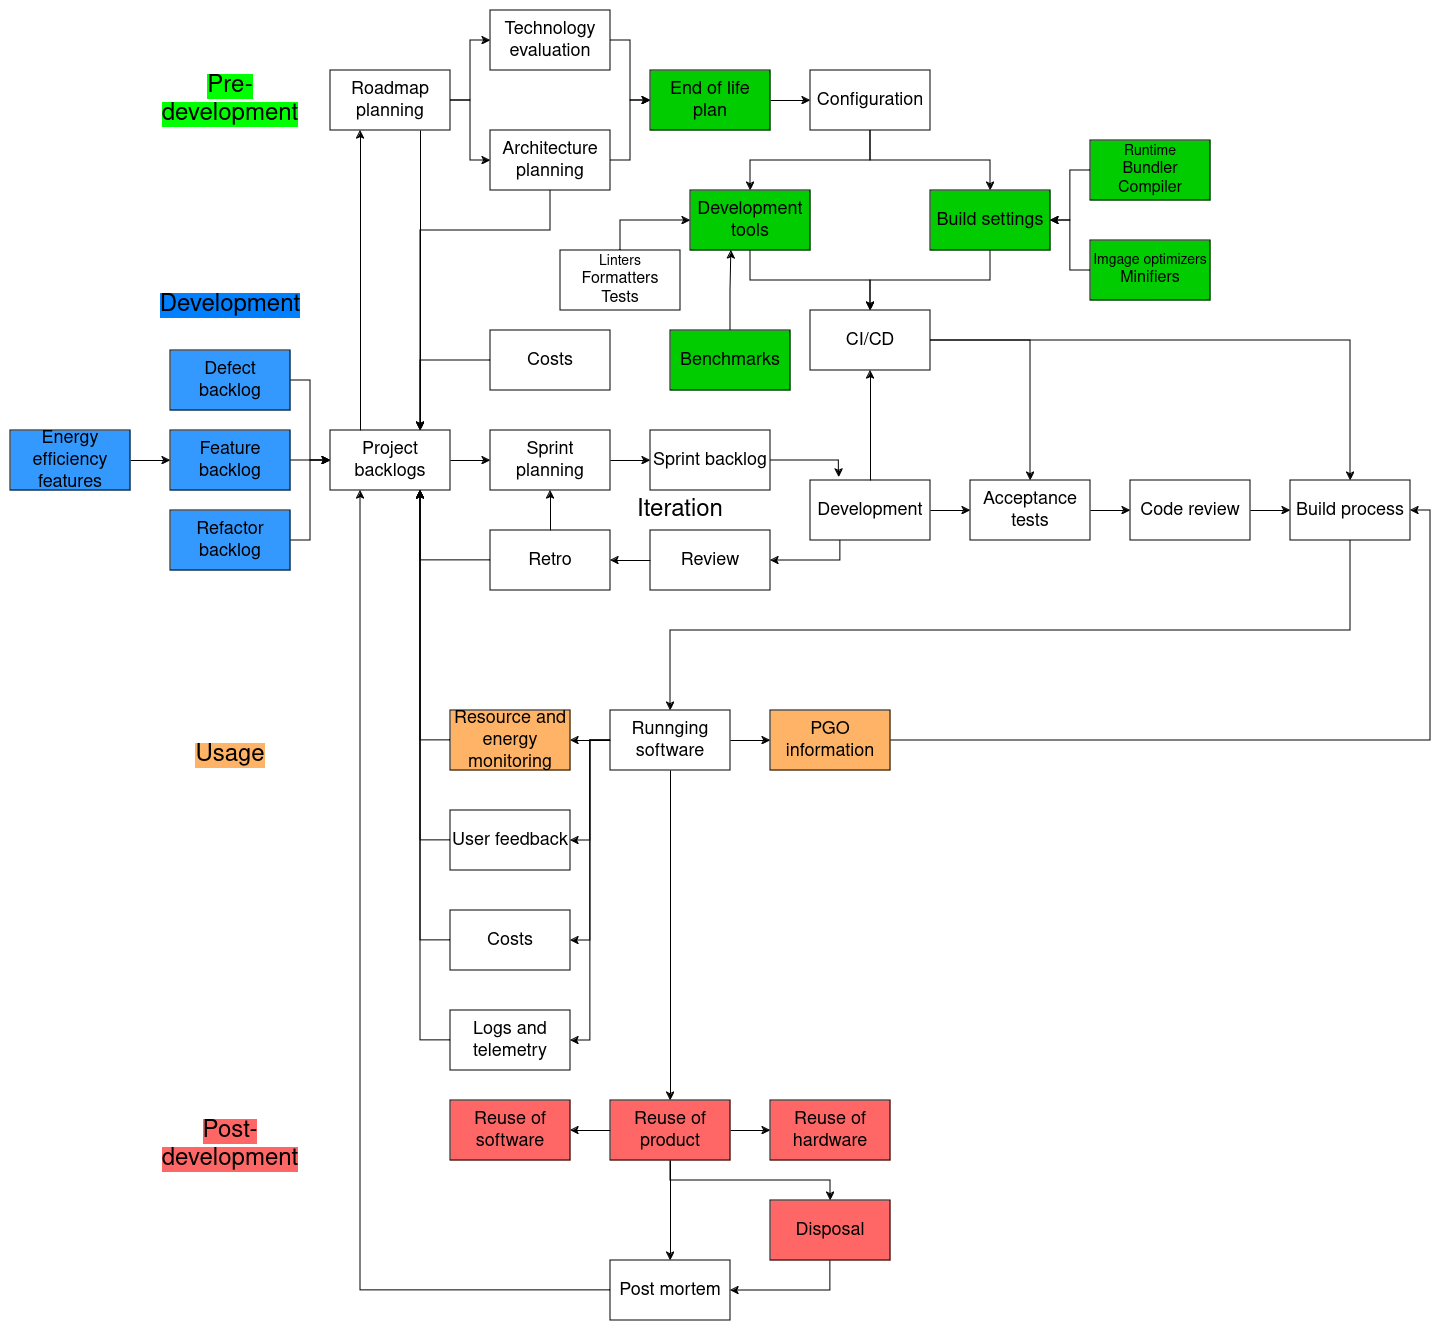
\includegraphics[width=\textwidth]{images/highlighted.png}
\centering
\caption{Highlighted additions of the proposed model}
\label{dev}
\end{figure}